% Options for packages loaded elsewhere
\PassOptionsToPackage{unicode}{hyperref}
\PassOptionsToPackage{hyphens}{url}
\PassOptionsToPackage{dvipsnames,svgnames,x11names}{xcolor}
%
\documentclass[
  12pt]{article}

\usepackage{amsmath,amssymb}
\usepackage{iftex}
\ifPDFTeX
  \usepackage[T1]{fontenc}
  \usepackage[utf8]{inputenc}
  \usepackage{textcomp} % provide euro and other symbols
\else % if luatex or xetex
  \usepackage{unicode-math}
  \defaultfontfeatures{Scale=MatchLowercase}
  \defaultfontfeatures[\rmfamily]{Ligatures=TeX,Scale=1}
\fi
\usepackage{lmodern}
\ifPDFTeX\else  
    % xetex/luatex font selection
\fi
% Use upquote if available, for straight quotes in verbatim environments
\IfFileExists{upquote.sty}{\usepackage{upquote}}{}
\IfFileExists{microtype.sty}{% use microtype if available
  \usepackage[]{microtype}
  \UseMicrotypeSet[protrusion]{basicmath} % disable protrusion for tt fonts
}{}
\makeatletter
\@ifundefined{KOMAClassName}{% if non-KOMA class
  \IfFileExists{parskip.sty}{%
    \usepackage{parskip}
  }{% else
    \setlength{\parindent}{0pt}
    \setlength{\parskip}{6pt plus 2pt minus 1pt}}
}{% if KOMA class
  \KOMAoptions{parskip=half}}
\makeatother
\usepackage{xcolor}
\setlength{\emergencystretch}{3em} % prevent overfull lines
\setcounter{secnumdepth}{5}
% Make \paragraph and \subparagraph free-standing
\makeatletter
\ifx\paragraph\undefined\else
  \let\oldparagraph\paragraph
  \renewcommand{\paragraph}{
    \@ifstar
      \xxxParagraphStar
      \xxxParagraphNoStar
  }
  \newcommand{\xxxParagraphStar}[1]{\oldparagraph*{#1}\mbox{}}
  \newcommand{\xxxParagraphNoStar}[1]{\oldparagraph{#1}\mbox{}}
\fi
\ifx\subparagraph\undefined\else
  \let\oldsubparagraph\subparagraph
  \renewcommand{\subparagraph}{
    \@ifstar
      \xxxSubParagraphStar
      \xxxSubParagraphNoStar
  }
  \newcommand{\xxxSubParagraphStar}[1]{\oldsubparagraph*{#1}\mbox{}}
  \newcommand{\xxxSubParagraphNoStar}[1]{\oldsubparagraph{#1}\mbox{}}
\fi
\makeatother


\providecommand{\tightlist}{%
  \setlength{\itemsep}{0pt}\setlength{\parskip}{0pt}}\usepackage{longtable,booktabs,array}
\usepackage{calc} % for calculating minipage widths
% Correct order of tables after \paragraph or \subparagraph
\usepackage{etoolbox}
\makeatletter
\patchcmd\longtable{\par}{\if@noskipsec\mbox{}\fi\par}{}{}
\makeatother
% Allow footnotes in longtable head/foot
\IfFileExists{footnotehyper.sty}{\usepackage{footnotehyper}}{\usepackage{footnote}}
\makesavenoteenv{longtable}
\usepackage{graphicx}
\makeatletter
\def\maxwidth{\ifdim\Gin@nat@width>\linewidth\linewidth\else\Gin@nat@width\fi}
\def\maxheight{\ifdim\Gin@nat@height>\textheight\textheight\else\Gin@nat@height\fi}
\makeatother
% Scale images if necessary, so that they will not overflow the page
% margins by default, and it is still possible to overwrite the defaults
% using explicit options in \includegraphics[width, height, ...]{}
\setkeys{Gin}{width=\maxwidth,height=\maxheight,keepaspectratio}
% Set default figure placement to htbp
\makeatletter
\def\fps@figure{htbp}
\makeatother

\addtolength{\oddsidemargin}{-.5in}%
\addtolength{\evensidemargin}{-1in}%
\addtolength{\textwidth}{1in}%
\addtolength{\textheight}{1.7in}%
\addtolength{\topmargin}{-1in}%
\makeatletter
\@ifpackageloaded{caption}{}{\usepackage{caption}}
\AtBeginDocument{%
\ifdefined\contentsname
  \renewcommand*\contentsname{Table of contents}
\else
  \newcommand\contentsname{Table of contents}
\fi
\ifdefined\listfigurename
  \renewcommand*\listfigurename{List of Figures}
\else
  \newcommand\listfigurename{List of Figures}
\fi
\ifdefined\listtablename
  \renewcommand*\listtablename{List of Tables}
\else
  \newcommand\listtablename{List of Tables}
\fi
\ifdefined\figurename
  \renewcommand*\figurename{Figure}
\else
  \newcommand\figurename{Figure}
\fi
\ifdefined\tablename
  \renewcommand*\tablename{Table}
\else
  \newcommand\tablename{Table}
\fi
}
\@ifpackageloaded{float}{}{\usepackage{float}}
\floatstyle{ruled}
\@ifundefined{c@chapter}{\newfloat{codelisting}{h}{lop}}{\newfloat{codelisting}{h}{lop}[chapter]}
\floatname{codelisting}{Listing}
\newcommand*\listoflistings{\listof{codelisting}{List of Listings}}
\makeatother
\makeatletter
\makeatother
\makeatletter
\@ifpackageloaded{caption}{}{\usepackage{caption}}
\@ifpackageloaded{subcaption}{}{\usepackage{subcaption}}
\makeatother
\ifLuaTeX
  \usepackage{selnolig}  % disable illegal ligatures
\fi
\usepackage[]{natbib}
\bibliographystyle{agsm}
\usepackage{bookmark}

\IfFileExists{xurl.sty}{\usepackage{xurl}}{} % add URL line breaks if available
\urlstyle{same} % disable monospaced font for URLs
\hypersetup{
  pdftitle={Compstak Analysis Progress},
  pdfauthor={William Clinton Co},
  colorlinks=true,
  linkcolor={blue},
  filecolor={Maroon},
  citecolor={Blue},
  urlcolor={Blue},
  pdfcreator={LaTeX via pandoc}}


\begin{document}


\def\spacingset#1{\renewcommand{\baselinestretch}%
{#1}\small\normalsize} \spacingset{1}


%%%%%%%%%%%%%%%%%%%%%%%%%%%%%%%%%%%%%%%%%%%%%%%%%%%%%%%%%%%%%%%%%%%%%%%%%%%%%%

\date{April 27, 2025}
\title{\bf Compstak Analysis Progress}
\author{
William Clinton Co\\
Department of Economics, University of British Columbia\\
}
\maketitle

\bigskip
\bigskip
\begin{abstract}
In this project, we conducted an initial review of the CompStak dataset
to assess its suitability for analyzing commercial properties in the
United States. Each field was individually evaluated, with a focus on
`Property Type' and `Property Subtype'. Our analysis revealed that while
fill rates for `Property Type' are high (95--99\%), `Property Subtype'
fields exhibit higher missingness (up to 28\%), potentially complicating
downstream analysis.We verified that property IDs are generally stable
across time and regions, although inconsistencies in property type and
subtype classifications were noted in a small fraction of records
(\textless0.02\%). To benchmark the dataset's coverage, we compared the
number of properties captured in CompStak against external (unverified)
estimates of U.S. commercial properties. Our findings indicate
non-uniform coverage across property types and states. Specifically,
industrial, office, and retail sectors are relatively well-represented,
whereas sectors like land and multifamily properties show significant
undercoverage. Geographically, West Coast states such as California show
higher representation, and regression analysis suggests that coverage
rates increase with the number of commercial properties in a given
state, indicating increasing returns to scale in data collection.
Challenges remain, particularly in mapping category definitions across
different datasets, such as the DOE and CoStar sources. Future work will
focus on improving benchmark estimates using the DOE dataset and
establishing a reliable mapping of property categories between datasets
to ensure meaningful comparisons.
\end{abstract}


\newpage
\spacingset{1.9} % DON'T change the spacing!

\section{Initial Analysis}\label{sec-intro}

Each field was reviewed individually to identify potential patterns, and
all fields appeared relevant for analysis. The broader data set includes
several types of industry classifications, such as `Property Type',
`Property Sub type', `Space Type', `Tenant SIC Code/Description', and
`Tenant NAICS Code/Description'. However, there is no clear
documentation explaining the differences between these classifications
or indicating which should be preferred. In our case, only `Property
Type' and `Property Sub type' are available, so our analysis will focus
on these variables. It is important to note that these classifications
are not consistently available across both lease and sales records,
which may introduce challenges to our analysis. Additionally, NAICS and
SIC codes are not included in our data set because they are a premium
add-on. Finally, `Space Type' is only available for lease data, which
may also pose limitations.

We observe ``fill rate'' (Table~\ref{tbl-one}), wherein a low fill rate
would correspond to a large portion of the entries having Nan or missing
values. Unique values shows us that the categories used for property
type and property sub type are consistent.

\begin{longtable}[]{@{}llll@{}}
\caption{Data set Initial Analysis}\label{tbl-one}\tabularnewline
\toprule\noalign{}
Data set & Type & Fill Rate & Unique Values \\
\midrule\noalign{}
\endfirsthead
\toprule\noalign{}
Data set & Type & Fill Rate & Unique Values \\
\midrule\noalign{}
\endhead
\bottomrule\noalign{}
\endlastfoot
Sales & Property type & 95\% & 8 \\
Lease & Property type & 99\% & 8 \\
Sales & Property Subtype & 75\% & 56 \\
Lease & Property Subtype & 66\% & 56 \\
\end{longtable}

We also investigate whether property IDs are consistent. We expect that
a given commercial property would exhibit stable characteristics, with
its location and industry classification remaining unchanged over time.
Our analysis confirms this expectation: property IDs are stable and pass
state consistency checks. However, it is important to note that property
types and sub types are not consistent. See Figure~\ref{fig-propertyid}
and Table~\ref{tbl-property_subtype}

\begin{figure}

\centering{

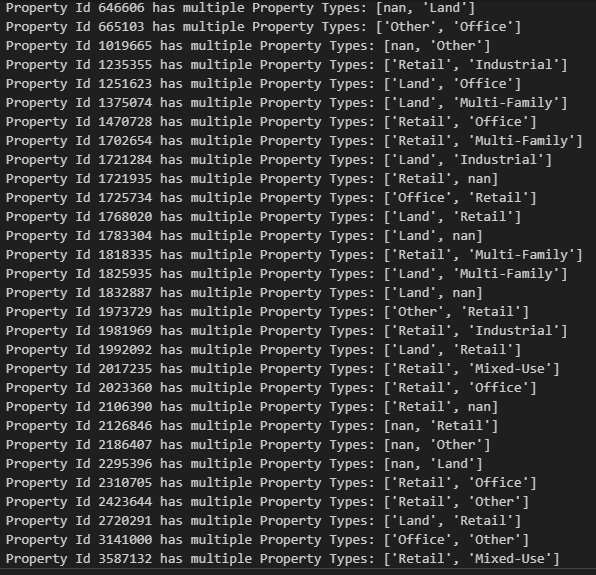
\includegraphics{images/Screenshot 2025-04-26 133959-01.png}

}

\caption{\label{fig-propertyid}Property ID Unstable Classifications}

\end{figure}%

Despite concerns about inconsistency, this is not a major issue, as the
number of unstable observations is relatively small compared to the
total number of properties. Specifically, property type inconsistency is
observed in only 39 cases, and property sub type inconsistency in 96
cases. This pales in comparison to the 759,623 unique properties in our
data set.

What is more concerning is the Nan surrounding each property type and
sub type. Wherein the Nan values for property sub types can be as high
as 28\% of the data. See Table~\ref{tbl-two}

\begin{longtable}[]{@{}
  >{\raggedright\arraybackslash}p{(\columnwidth - 6\tabcolsep) * \real{0.2603}}
  >{\raggedright\arraybackslash}p{(\columnwidth - 6\tabcolsep) * \real{0.2603}}
  >{\raggedright\arraybackslash}p{(\columnwidth - 6\tabcolsep) * \real{0.2192}}
  >{\raggedright\arraybackslash}p{(\columnwidth - 6\tabcolsep) * \real{0.2603}}@{}}
\caption{Error Associated with Property
Types}\label{tbl-two}\tabularnewline
\toprule\noalign{}
\begin{minipage}[b]{\linewidth}\raggedright
Error Type
\end{minipage} & \begin{minipage}[b]{\linewidth}\raggedright
Industry Category Type
\end{minipage} & \begin{minipage}[b]{\linewidth}\raggedright
Number
\end{minipage} & \begin{minipage}[b]{\linewidth}\raggedright
Percentage
\end{minipage} \\
\midrule\noalign{}
\endfirsthead
\toprule\noalign{}
\begin{minipage}[b]{\linewidth}\raggedright
Error Type
\end{minipage} & \begin{minipage}[b]{\linewidth}\raggedright
Industry Category Type
\end{minipage} & \begin{minipage}[b]{\linewidth}\raggedright
Number
\end{minipage} & \begin{minipage}[b]{\linewidth}\raggedright
Percentage
\end{minipage} \\
\midrule\noalign{}
\endhead
\bottomrule\noalign{}
\endlastfoot
Inconsistent Category & Property Type & 39 / 759623 & 0.00513\% \\
Inconsistent Category & Property Subtype & 96 / 759623 & 0.01264\% \\
Nan & Property Type & 37020 / 759623 & 4.87\% \\
Nan & Property Subtype & 213255 / 759623 & 28.07\% \\
\end{longtable}

\section{Strategy}\label{strategy}

We will begin by matching the number of buildings. Specifically, we
observe unique property IDs in the data set, allowing us to estimate the
number of commercial properties in the United States. The total number
of commercial properties is a relatively stable metric to study compared
to more volatile measures such as valuations or square footage.

Using this approach, we can first compare aggregate numbers, starting
with the total number of properties in the United States, and then work
our way downward to industry-level and state-level comparisons.

We first assess how much of the national commercial property market is
captured in our data set. We assume that the CompStak data set
represents only a small subsection of the total U.S. market. However, a
key concern is whether these observations are uniformly distributed
across regions and industries, or if there are systematic biases. For
example, are retail properties in California more likely to be reported
than warehouses in Michigan?

To begin, we pull external estimates of the total number of commercial
properties from publicly available internet sources. Although these
external figures are unverified, they provide a useful starting point
for benchmarking and analyzing the coverage of our data set. See
Table~\ref{tbl-Industry} and Table~\ref{tbl-State}

\section{Results}\label{results}

The following analysis uses unverified U.S. figures. We observe evidence
of non-uniform coverage. If we assume the complete circle represents the
true total number of U.S. commercial properties, then the CompStak data
represents a subsample of this total. The ``Covered'' section reflects
properties captured in the CompStak dataset, while the ``Gap''
represents the ``missing'' properties not covered.

As shown in Figure~\ref{fig-sunburst1} , office, industrial, and retail
sectors appear relatively well covered. Industrial coverage is
approximately 53\%, while office and retail each have around 22\%
coverage. Coverage for the remaining sectors is negligible, with less
than 5\% represented.

\begin{figure}

\centering{

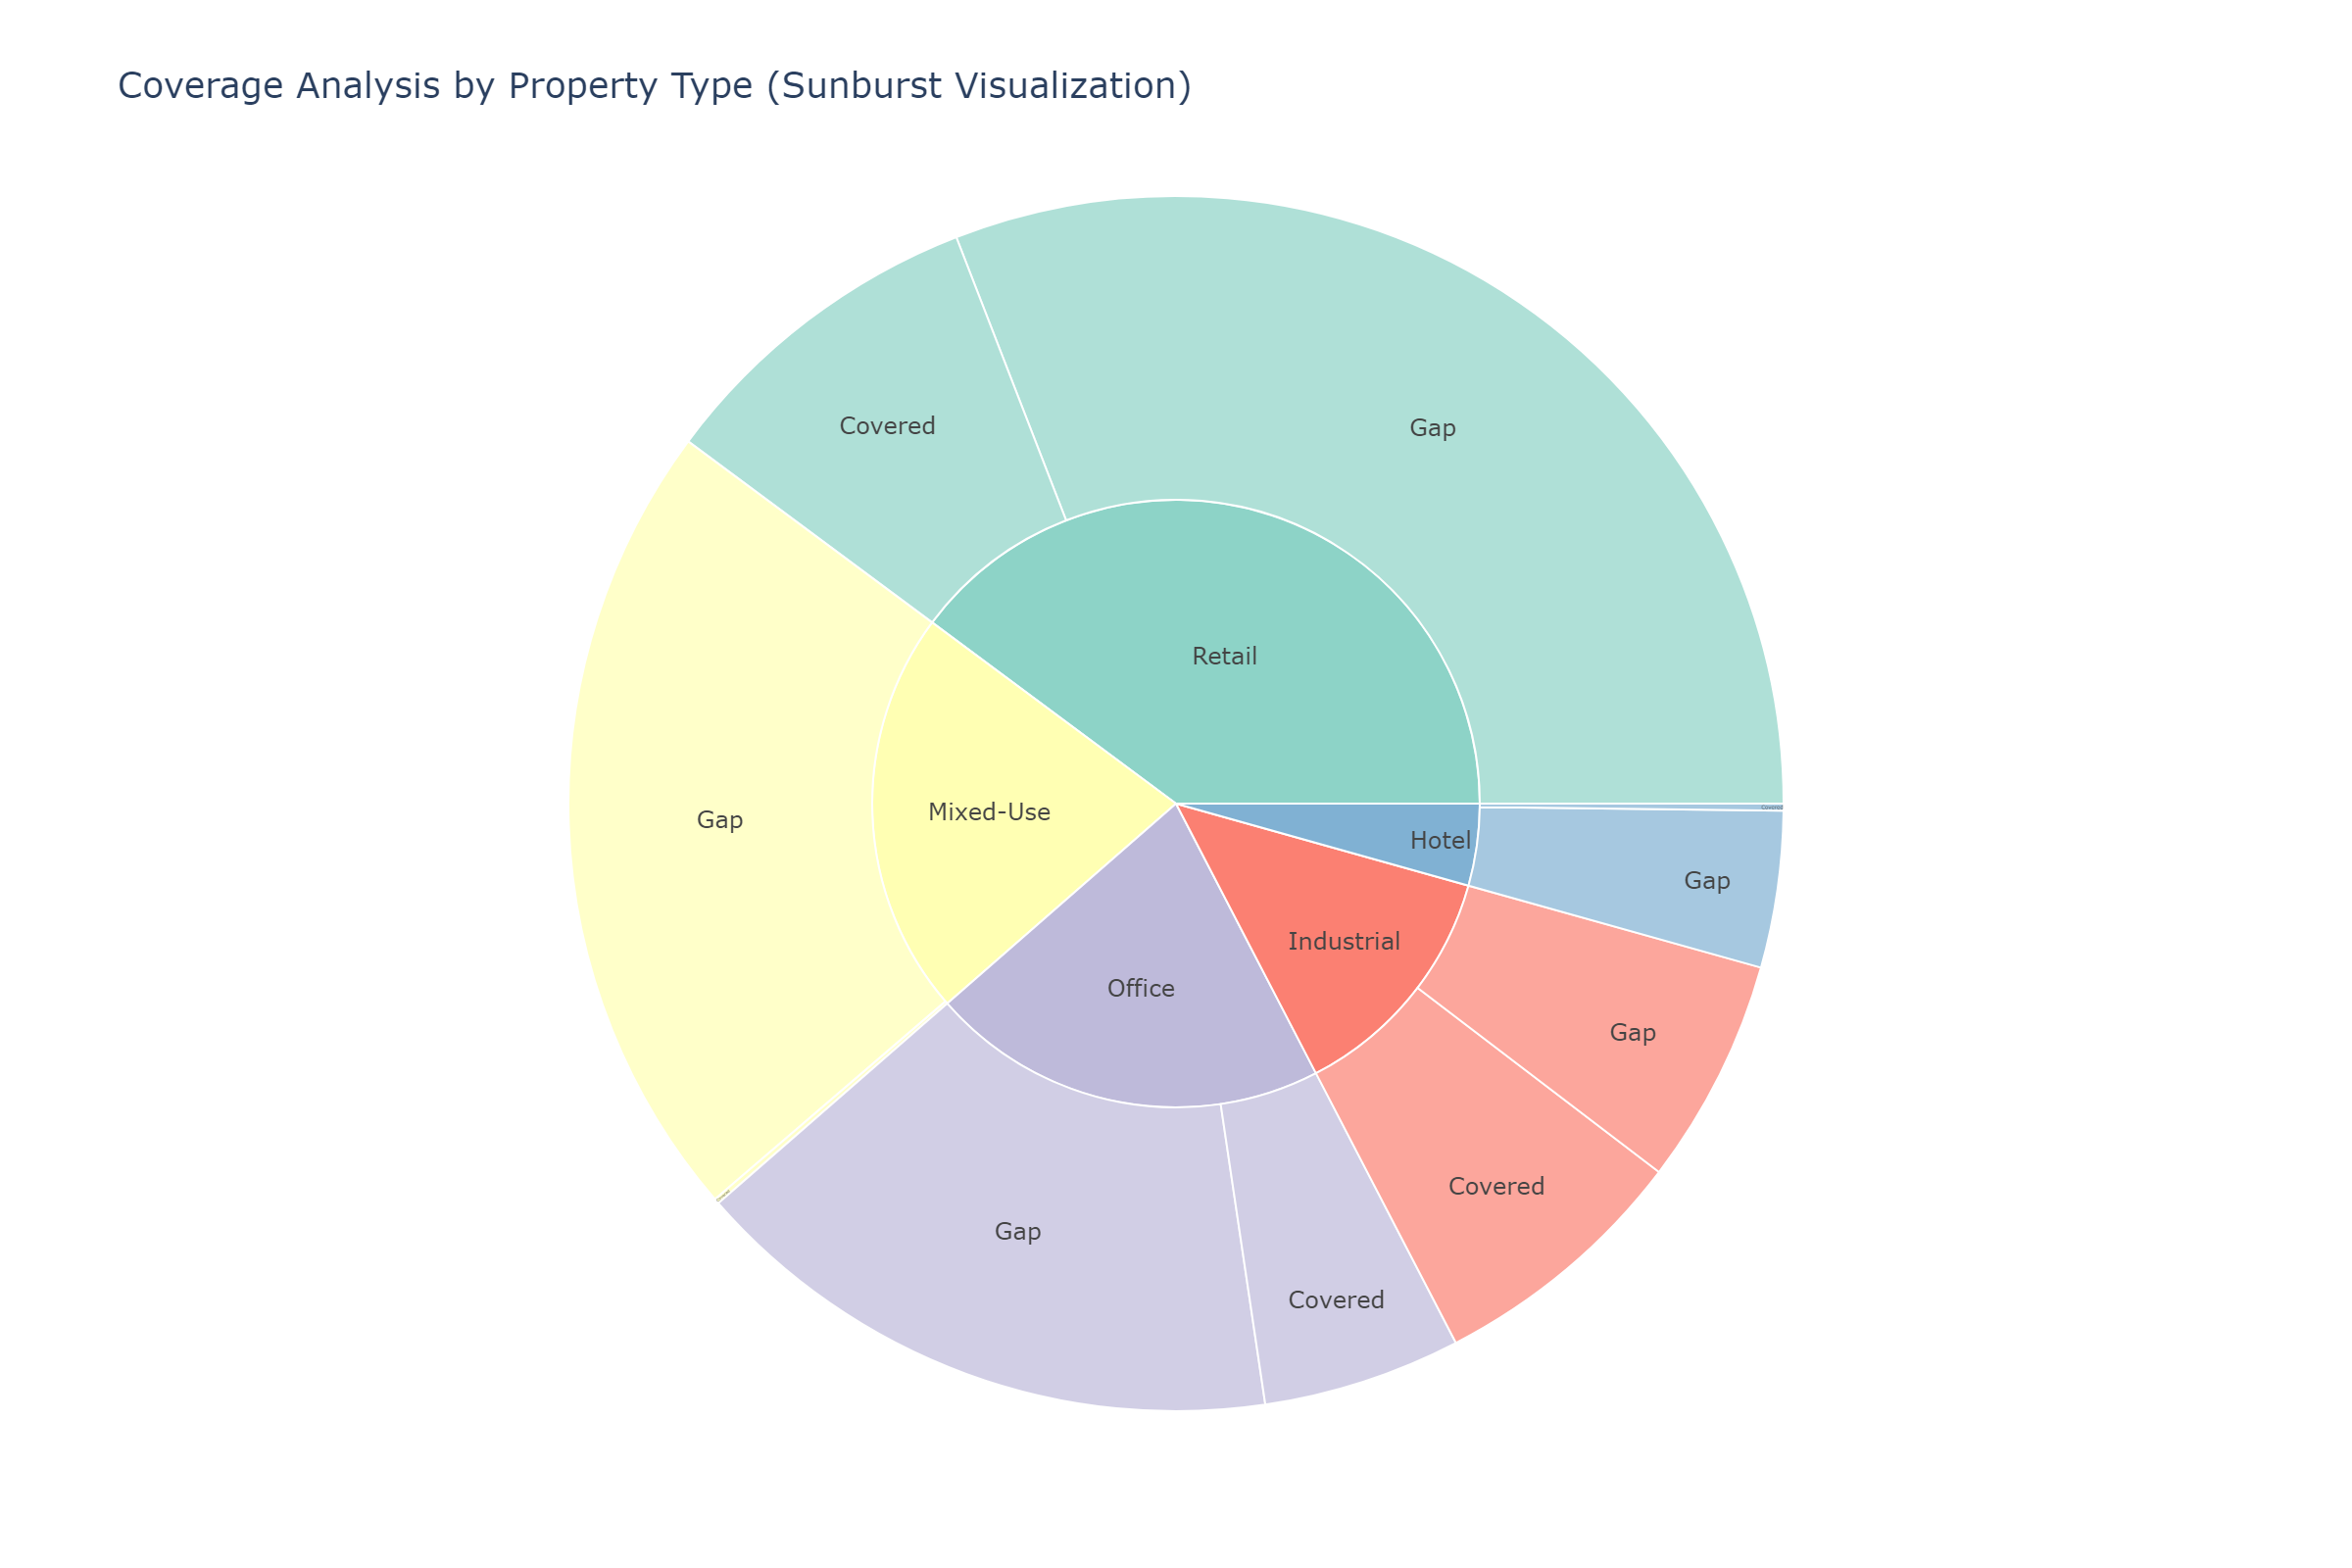
\includegraphics{images/filtered_coverage_sunburst_20250424_234213.png}

}

\caption{\label{fig-sunburst1}}

\end{figure}%

In particular see Figure~\ref{fig-sunburst2} see that land and
multi-family have extremely low coverage, at the same time representing
a large portion of total US commercial properties.

\begin{figure}

\centering{

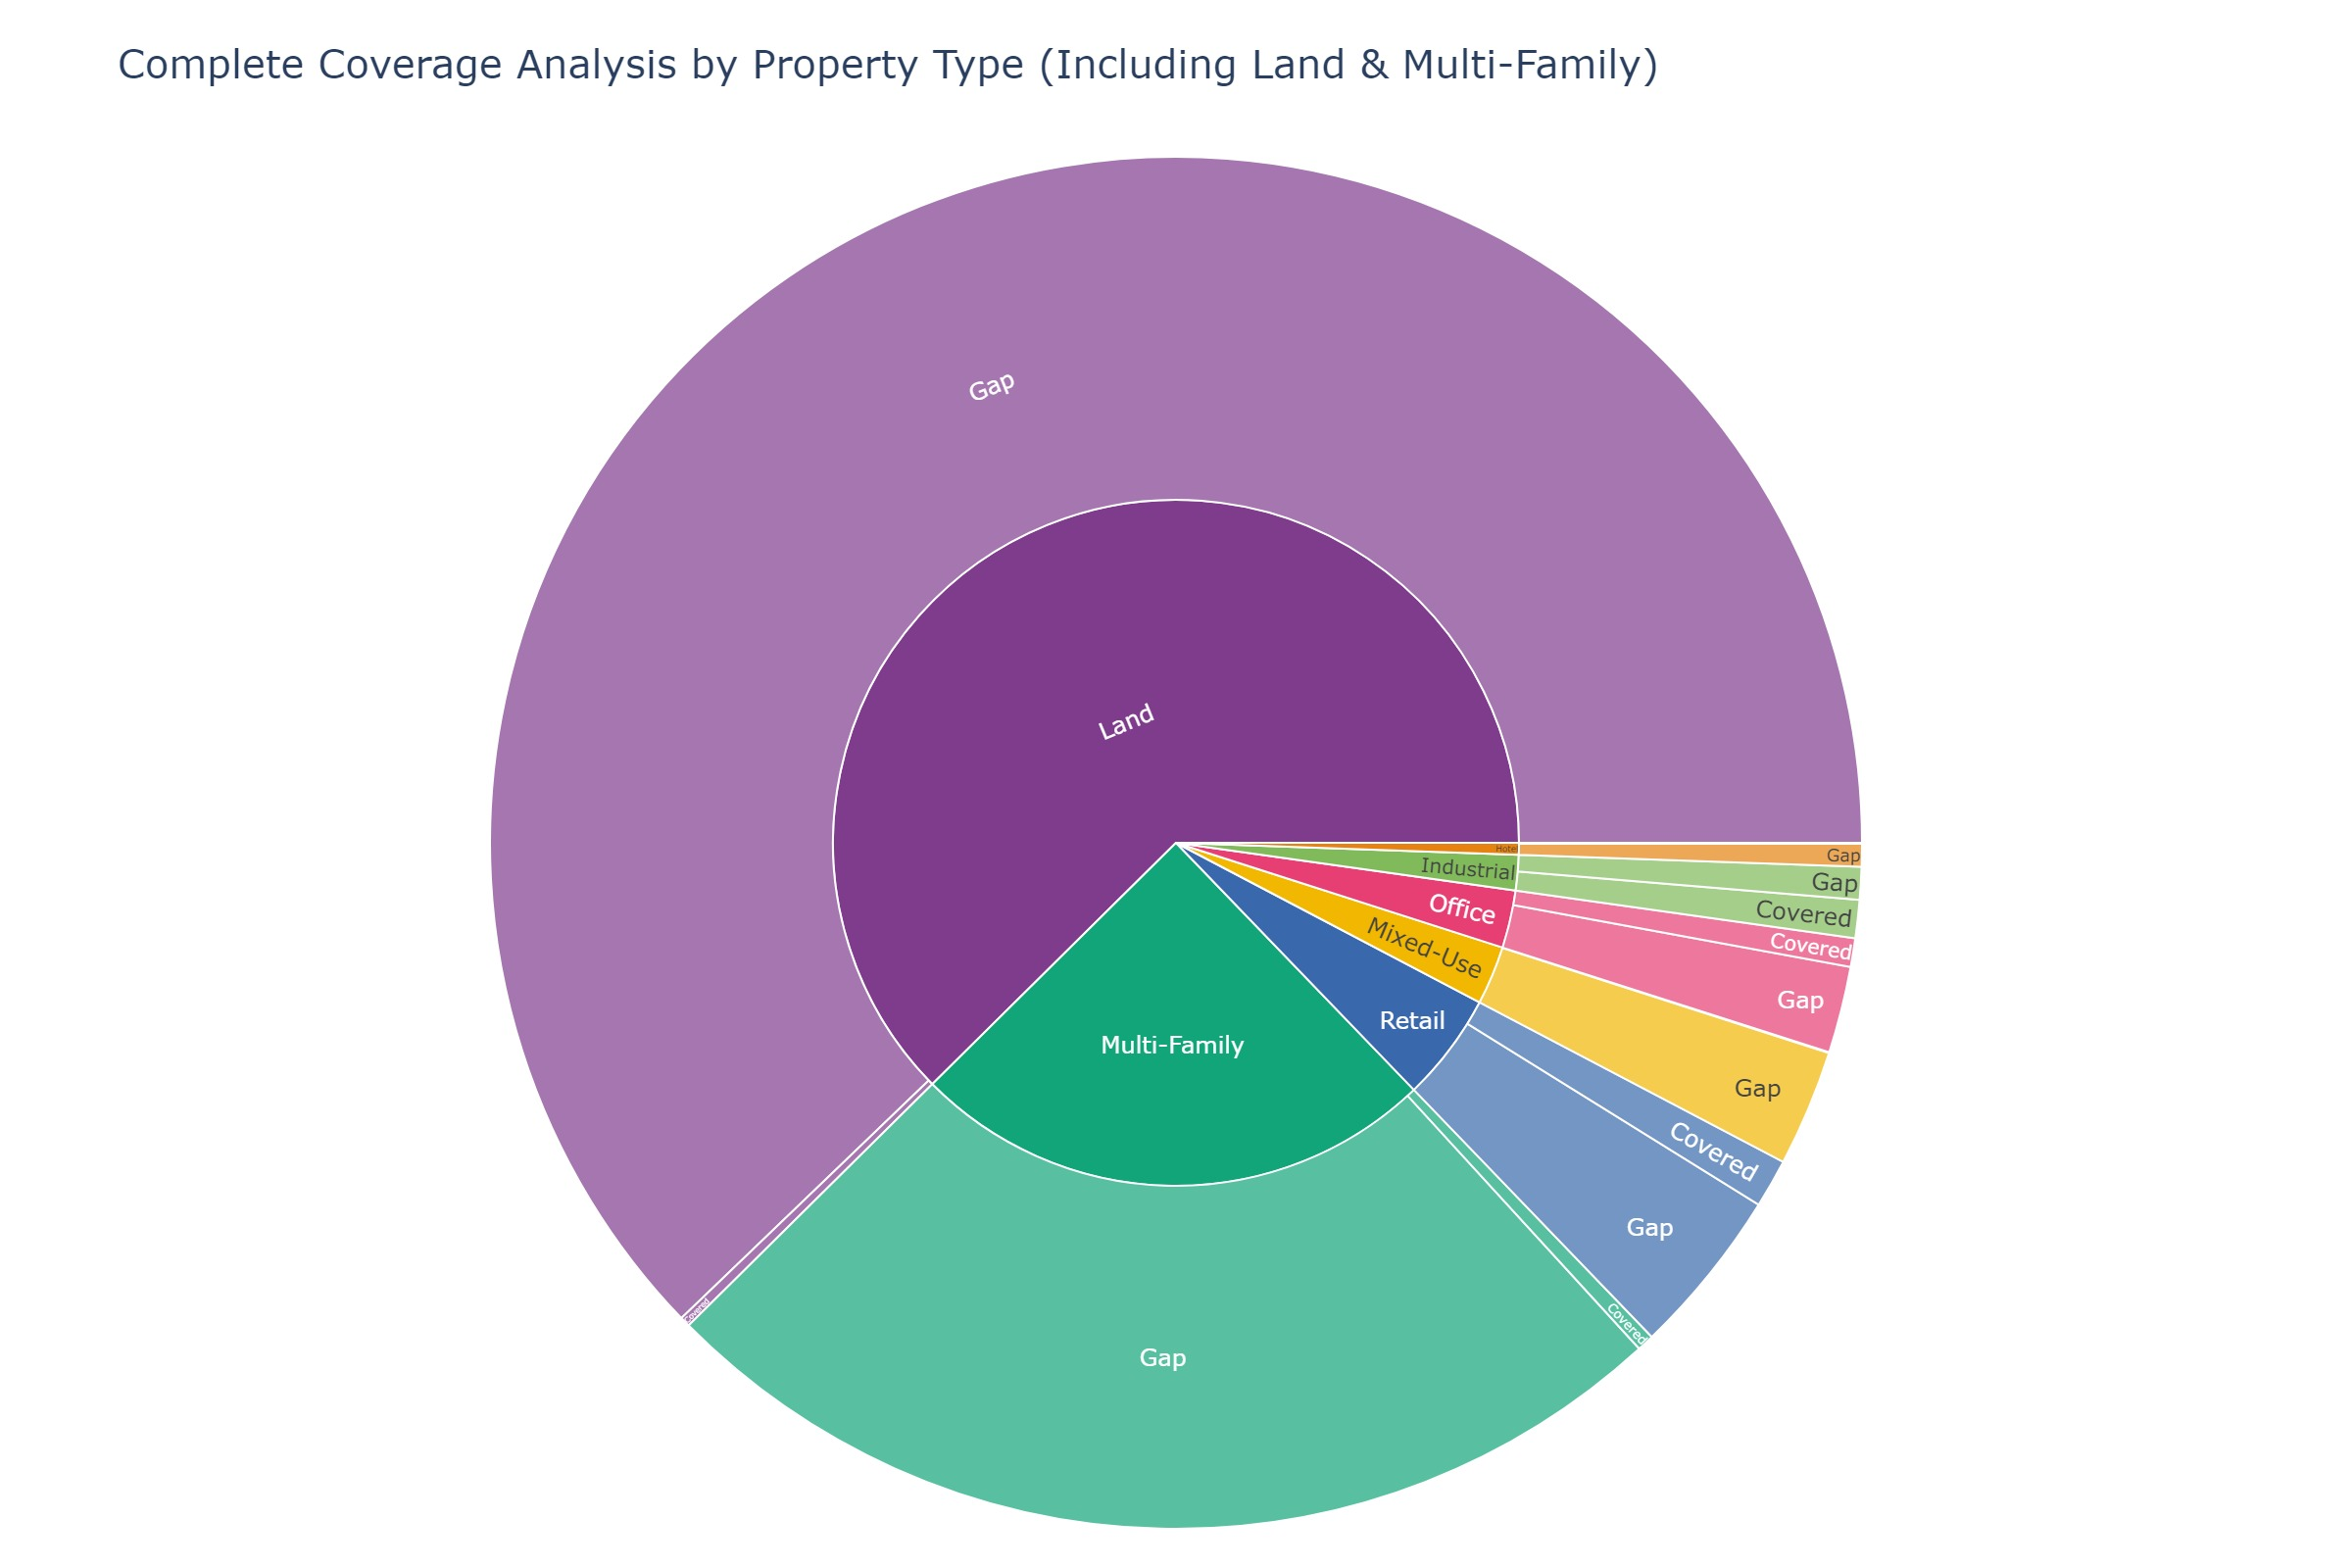
\includegraphics{images/complete_coverage_sunburst_20250425_110035.jpg}

}

\caption{\label{fig-sunburst2}}

\end{figure}%

Using the same data set, I investigated the uniformity of coverage
across states. The analysis reveals that the CompStak dataset exhibits a
bias toward West Coast states. As shown in Figure~\ref{fig-map}, the
coverage rate is calculated by assuming the externally sourced U.S. data
set estimate provides the true number of commercial properties, with the
CompStak dataset representing a subset. For example, California has an
18\% coverage rate, meaning that the number of commercial property
observations in CompStak accounts for 18\% of the estimated 917,860
commercial properties in California.

\begin{figure}

\centering{

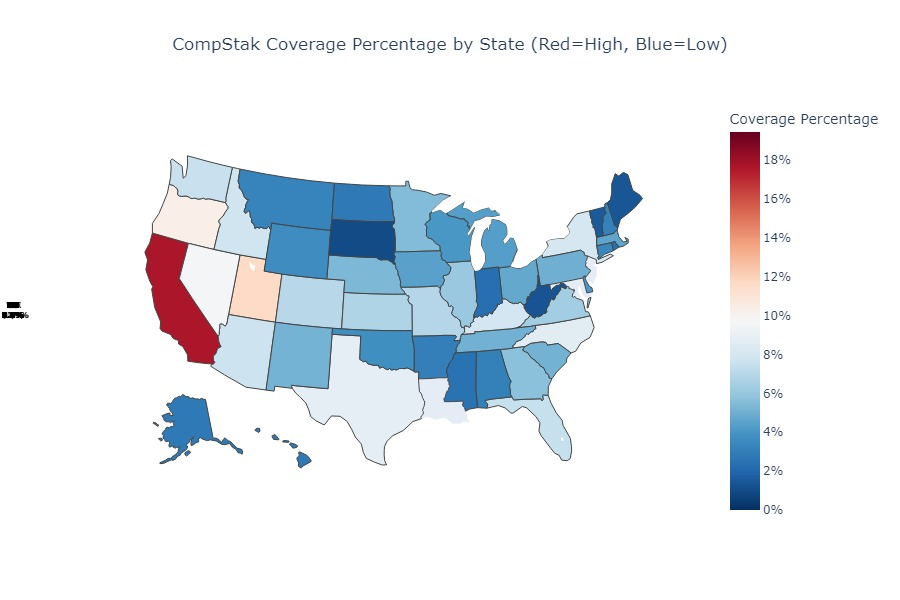
\includegraphics{images/coverage_percentage_redblue_20250425_010815.jpg}

}

\caption{\label{fig-map}}

\end{figure}%

Next, we examine the determinants of this observation. Specifically, I
assess whether the coverage rate is a function of the total number of
commercial properties in each state, again assuming that our U.S.
estimate represents the true total. As shown in Figure~\ref{fig-prop1},
there is evidence to support this theory. States with a greater number
of commercial properties tend to have higher coverage rates in the
CompStak dataset, as indicated by the linear regression results in
Figure~\ref{fig-prop1}. This pattern suggests that there are fixed costs
associated with data collection in each location, and that data
providers are more likely to specialize in areas with larger commercial
markets. As a result, the dataset exhibits increasing returns to scale,
which introduces bias into our observations.

\begin{figure}

\centering{

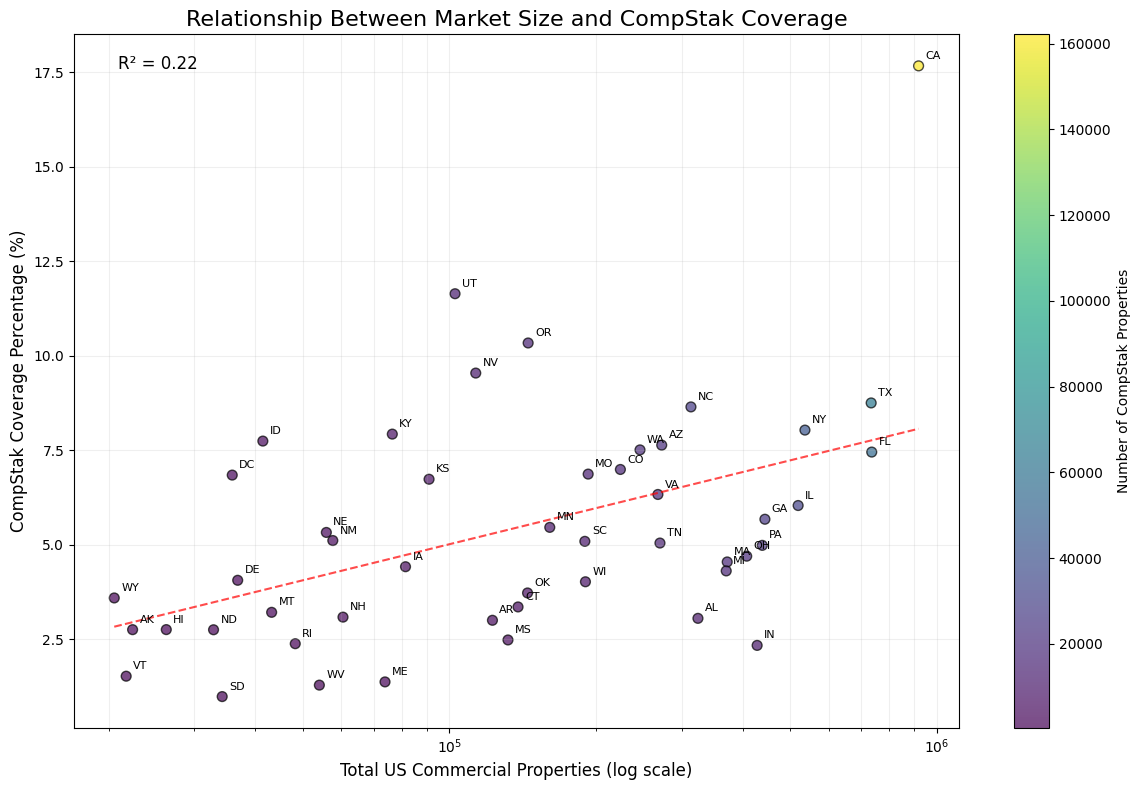
\includegraphics{images/7.png}

}

\caption{\label{fig-prop1}}

\end{figure}%

A similar analysis was conducted using property types, but several
challenges were encountered. Specifically, the top two outliers
significantly skewed the regression line, suggesting potential issues
with category interpretation or data quality. Further investigation is
warranted to better understand these anomalies. However, it is
noteworthy that when these outliers are excluded, the regression line
again shows a positive relationship: property types with more commercial
properties tend to have higher CompStak coverage rates. The
corresponding graph can be found in the appendix. Figure~\ref{fig-prop2}
Figure~\ref{fig-prop3}

\section{Concluding Thoughts}\label{concluding-thoughts}

NAICS and SIC codes may be worth considering, given their standardized
format and consistency across multiple datasets, depending on our
analytical needs. We also realized that our observations may be biased
due to unverified numbers in our current data set. Therefore, to ensure
greater accuracy, we will be studying the DOE dataset of estimated
numbers of commercial properties in the United States
(\href{https://www.costar.com/about/costar-glossary}{CoStar Glossary},
\href{https://catalog.data.gov/dataset/city-and-county-commercial-building-inventories-010d2}{DOE
Dataset}).

While this is a good starting point, it will require significant effort
to reliably reproduce our unverified US estimate data using the DOE
dataset. Determining the appropriate mapping and definitions takes time.
For example, the DOE categorizes commercial properties under terms such
as ``sports and entertainment'' or ``specialty,'' which may not directly
correspond to the categories used in the CompStak dataset. The
\href{https://www.costar.com/about/costar-glossary}{CoStar Glossary}
provides definitions for some of these categories, and a comparison with
Table~\ref{tbl-Industry} in our dataset highlights these differences.
This underscores the need for careful mapping and interpretation when
aligning categories across datasets.

A careful review of category definitions and thoughtful value judgments
will be necessary to establish equivalencies and ensure meaningful
comparisons in our analysis. Additionally, it would be beneficial to
determine whether a comprehensive glossary of categories exists for the
CompStak dataset. To the best of my knowledge, there is currently no
CompStak glossary that is directly comparable to the
\href{https://www.costar.com/about/costar-glossary}{CoStar Glossary}.

\section{Appendix}\label{appendix}

\begin{figure}

\centering{

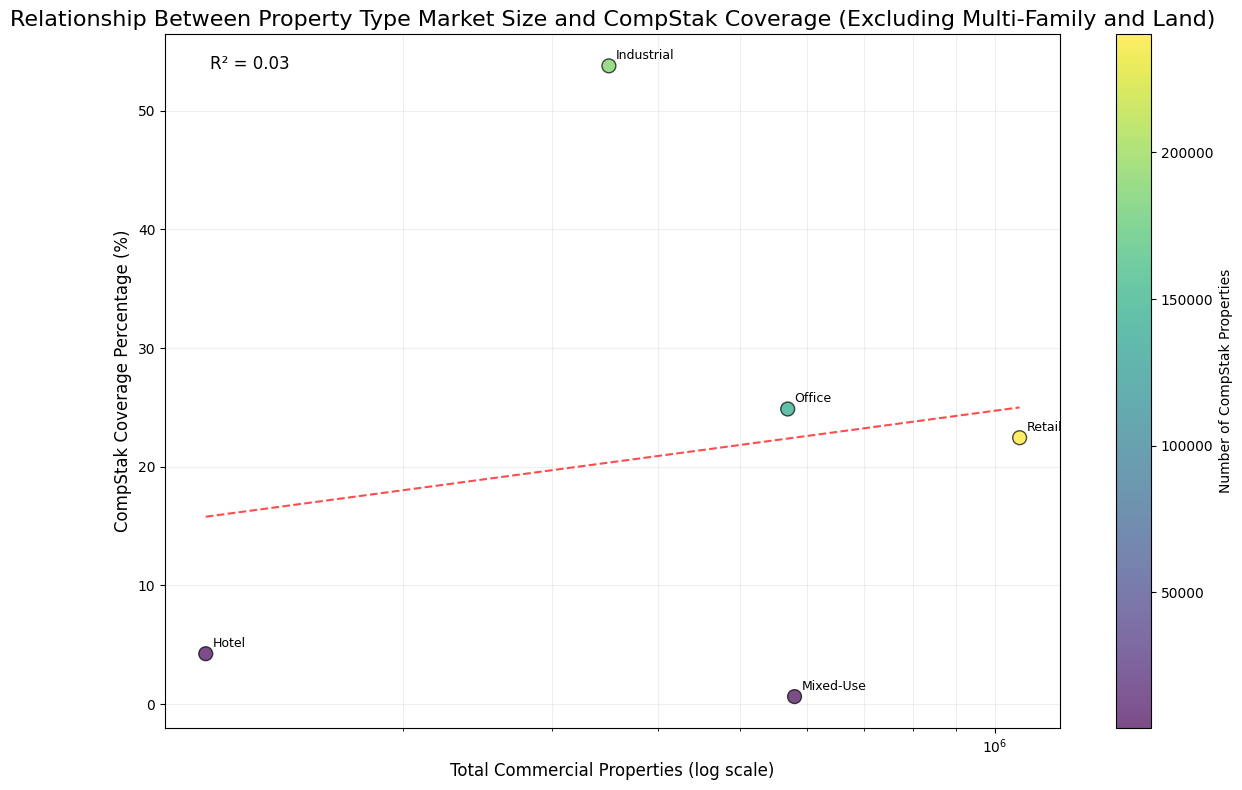
\includegraphics{images/8.png}

}

\caption{\label{fig-prop2}}

\end{figure}%

\begin{figure}

\centering{

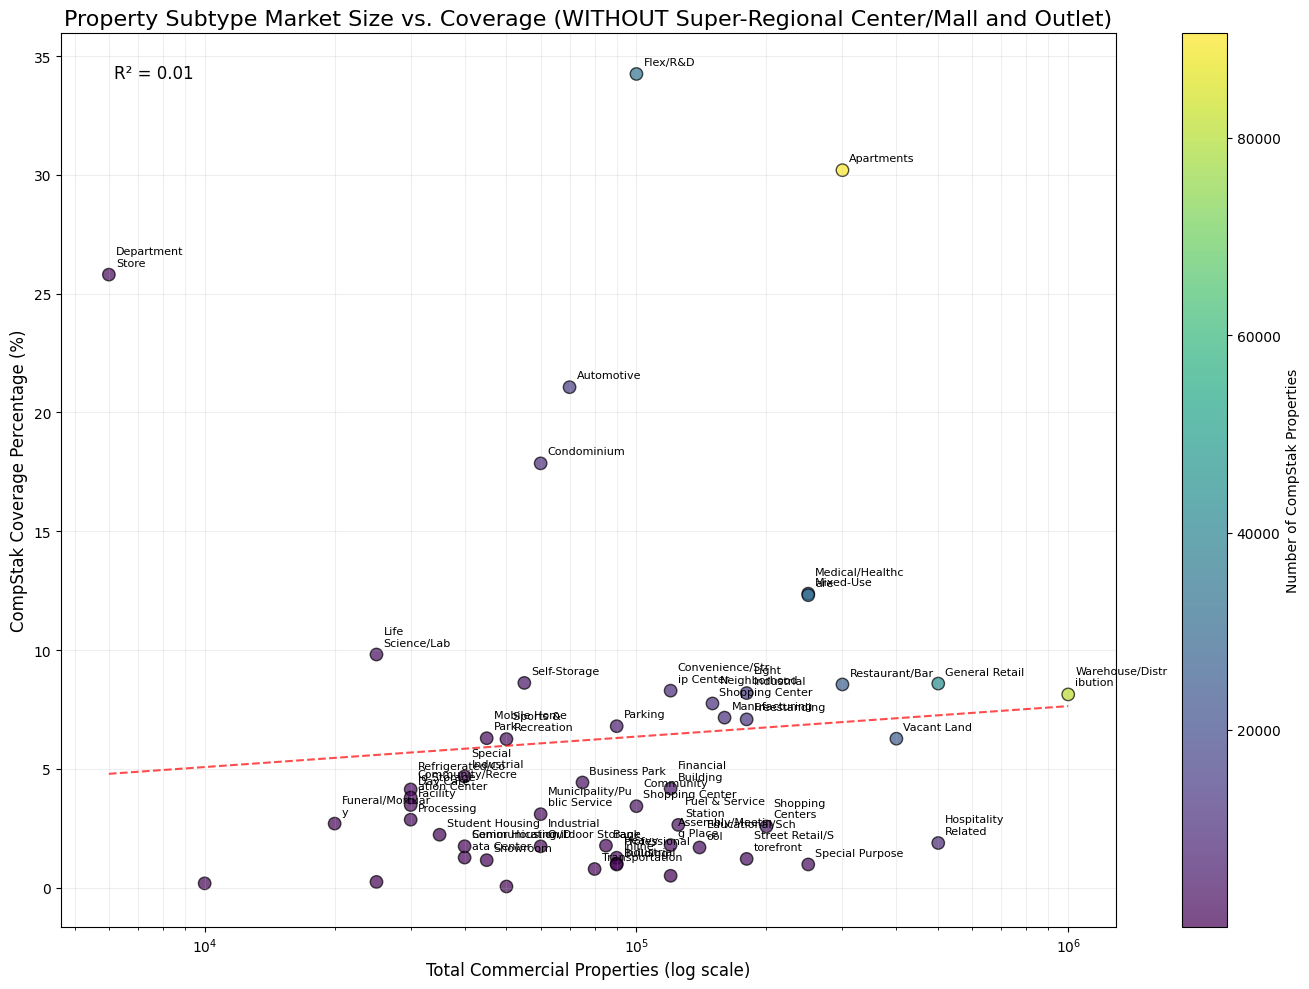
\includegraphics{images/9.png}

}

\caption{\label{fig-prop3}}

\end{figure}%

\begin{longtable}[]{@{}ll@{}}
\caption{Number of Commercial Properties by Industry (Unverified
Internet Sourced US estimates)}\label{tbl-Industry}\tabularnewline
\toprule\noalign{}
Property Type & Estimated Number of Properties \\
\midrule\noalign{}
\endfirsthead
\toprule\noalign{}
Property Type & Estimated Number of Properties \\
\midrule\noalign{}
\endhead
\bottomrule\noalign{}
\endlastfoot
Retail & 1,070,000 \\
Industrial & 350,000 \\
Office & 569,311 \\
Multi-Family & 5,200,000 \\
Hotel & 116,873 \\
Mixed-Use & 580,000 \\
Land & 13,100,000 \\
Other & Not specified \\
\end{longtable}

\begin{longtable}[]{@{}ll@{}}
\caption{Number of Commercial Properties by State (Unverified Internet
Sourced US estimates)}\label{tbl-State}\tabularnewline
\toprule\noalign{}
State & Commercial Properties \\
\midrule\noalign{}
\endfirsthead
\toprule\noalign{}
State & Commercial Properties \\
\midrule\noalign{}
\endhead
\bottomrule\noalign{}
\endlastfoot
CA & 917,860 \\
TX & 733,648 \\
FL & 735,652 \\
NY & 536,608 \\
IL & 519,616 \\
PA & 438,648 \\
OH & 407,557 \\
GA & 444,143 \\
NC & 313,187 \\
MI & 369,983 \\
WA & 246,208 \\
AZ & 272,797 \\
MA & 371,710 \\
VA & 267,936 \\
CO & 224,418 \\
IN & 428,138 \\
TN & 270,544 \\
MO & 192,733 \\
WI & 190,274 \\
MN & 160,773 \\
AL & 323,716 \\
SC & 189,736 \\
KY & 76,415 \\
OR & 145,157 \\
OK & 144,752 \\
CT & 138,387 \\
IA & 81,338 \\
MS & 131,969 \\
AR & 122,634 \\
KS & 90,904 \\
NV & 113,336 \\
UT & 102,769 \\
NM & 57,693 \\
NE & 55,961 \\
WV & 54,143 \\
ID & 41,460 \\
HI & 26,275 \\
ME & 73,831 \\
NH & 60,537 \\
RI & 48,317 \\
MT & 43,219 \\
DE & 36,816 \\
SD & 34,215 \\
ND & 32,846 \\
AK & 22,410 \\
VT & 21,740 \\
WY & 20,549 \\
DC & 35,878 \\
\end{longtable}

\section{}\label{section}

\begin{longtable}[]{@{}
  >{\raggedright\arraybackslash}p{(\columnwidth - 2\tabcolsep) * \real{0.1831}}
  >{\raggedright\arraybackslash}p{(\columnwidth - 2\tabcolsep) * \real{0.8169}}@{}}
\caption{Property Sub type
Inconsistency}\label{tbl-property_subtype}\tabularnewline
\toprule\noalign{}
\begin{minipage}[b]{\linewidth}\raggedright
Property ID
\end{minipage} & \begin{minipage}[b]{\linewidth}\raggedright
Inconsistent Property Subtypes
\end{minipage} \\
\midrule\noalign{}
\endfirsthead
\toprule\noalign{}
\begin{minipage}[b]{\linewidth}\raggedright
Property ID
\end{minipage} & \begin{minipage}[b]{\linewidth}\raggedright
Inconsistent Property Subtypes
\end{minipage} \\
\midrule\noalign{}
\endhead
\bottomrule\noalign{}
\endlastfoot
21036 & General Retail, nan \\
353844 & nan, Vacant Land \\
354461 & nan, Municipality/Public Service \\
374802 & nan, Vacant Land \\
398906 & nan, Vacant Land \\
415099 & General Retail, nan \\
418514 & Apartments, Sports \& Recreation \\
420902 & nan, Apartments \\
422199 & Outlet, Vacant Land \\
433935 & nan, Municipality/Public Service \\
434400 & nan, Vacant Land \\
443800 & Vacant Land, Super-Regional Center/Mall \\
444319 & Apartments, nan \\
445159 & General Retail, nan \\
448126 & Apartments, nan \\
449199 & General Retail, nan \\
466525 & General Retail, nan \\
476566 & Parking, Apartments \\
485298 & nan, Shopping Centers \\
489216 & nan, Parking \\
490863 & nan, Automotive \\
491210 & Apartments, General Retail \\
491863 & Apartments, Vacant Land \\
496416 & nan, Apartments \\
508849 & General Retail, Shopping Centers \\
520174 & nan, Vacant Land \\
538162 & Vacant Land, nan \\
567596 & Super-Regional Center/Mall, Neighborhood Shopping Center \\
581027 & nan, General Retail \\
581309 & Apartments, nan \\
623357 & Vacant Land, nan \\
624813 & Condominium, Apartments \\
633831 & Apartments, nan \\
646161 & General Retail, nan \\
669817 & nan, Apartments \\
679028 & Apartments, nan \\
699484 & nan, Apartments \\
702675 & Apartments, nan \\
703449 & nan, Apartments \\
731139 & Apartments, Convenience/Strip Center \\
742440 & nan, Apartments \\
745417 & Vacant Land, nan \\
754857 & nan, Apartments \\
755143 & General Retail, nan \\
757418 & Apartments, nan \\
849172 & Flex/R\&D, Business Park \\
1204302 & General Retail, nan \\
1211995 & nan, Sports \& Recreation \\
1212507 & Special Purpose, nan \\
1235355 & General Retail, Vacant Land \\
1254651 & Self-Storage, nan \\
1255443 & Vacant Land, Condominium \\
1261872 & nan, Mixed-Use \\
1272015 & Freestanding, General Retail \\
1311302 & General Retail, Freestanding \\
1418012 & Warehouse/Distribution, Special Industrial \\
1421693 & Apartments, nan \\
1431770 & nan, Vacant Land \\
1448113 & nan, General Retail \\
1449588 & Apartments, Financial Building \\
1451345 & nan, Apartments \\
1684081 & nan, Light Industrial \\
1705515 & Manufacturing, Light Industrial \\
1721935 & Day Care Facility, nan \\
1722765 & Super-Regional Center/Mall, Convenience/Strip Center \\
1724884 & Vacant Land, nan \\
1725903 & General Retail, Community Shopping Center \\
1743582 & nan, General Retail \\
1765432 & Apartments, nan \\
1822722 & Vacant Land, nan \\
1858406 & nan, Apartments \\
1866157 & Hospitality Related, Apartments \\
1922481 & nan, Apartments \\
1929300 & Condominium, nan \\
2049015 & General Retail, nan \\
2050907 & Apartments, nan \\
2054074 & nan, Super-Regional Center/Mall \\
2057688 & nan, Vacant Land \\
2096757 & nan, Vacant Land \\
2106390 & Automotive, nan \\
2144456 & Parking, Restaurant/Bar \\
2266042 & Apartments, nan \\
2288779 & Parking, Warehouse/Distribution \\
2292241 & nan, Warehouse/Distribution \\
2295396 & nan, Vacant Land \\
2330278 & Apartments, nan \\
2331364 & Vacant Land, General Retail \\
2423080 & nan, Vacant Land \\
2425229 & nan, Restaurant/Bar \\
2720291 & Vacant Land, Mixed-Use \\
3417569 & nan, Medical/Healthcare \\
3417659 & nan, Mixed-Use \\
3418319 & nan, Mixed-Use \\
3464690 & Warehouse/Distribution, Manufacturing \\
3575908 & Community Shopping Center, Vacant Land \\
3587132 & Apartments, Mixed-Use \\
\end{longtable}


  \bibliography{bibliography.bib}


\end{document}
